\subsection{Design, comparators and service endpoints}
Three complementary studies test the coordination under unchanged
selected tasks. Core factorial controls isolate whether retained
computation becomes continuously available service [EL]/[SUP]. Native
tests ask whether early complete calls preserve the original recursively
selected task [EL]/[AU]. Process-failure tests distinguish already
accepted results from future message authority. Their benefits arise
under different execution contracts and are evaluated separately.
An instrumented FIFO Consumer records actual applications. All accepted
inputs keep their original ready times through cancellation and recovery.

\paragraph{Core implementation and sources}
Two 24-GB RTX~3090s host an FP16 Private worker and FP32 Authority worker.
Qwen3-ASR~1.7B~\cite{shi2026qwen3asr} is primary; Whisper base.en
\cite{radford2023whisper} tests a second state adapter. Complete-row
delivery, at most 16 rows per batch, a 256-token limit, the protocol kernel
and synchronized journals are shared. Physical early exit is disabled
in this factorial study, separating retention from cancellation.
Initial loading precedes the service clock. Energy integrates both
physical boards over the declared service window.

Independent confirmation uses 24 previously unused LibriSpeech speakers
\cite{panayotov2015librispeech}, metadata-selected before inference and
partitioned into three eight-speaker cohorts, totaling 714.110~s per arm.
Its 110 cells cover primary controls, fresh-process repeats and coarser
feedback schedules. At $\rho=1$, Authority advances every 2~s;
$\rho=3$ changes selection frequency and feedback segmentation. Arrivals
are simultaneous or staggered by 0.25~s. We reuse public recordings without
collecting participant data; repetitions share speakers, the independent
acoustic units.

\paragraph{Named comparisons}
\emph{Checked snapshot + recomputation} ($R_0S_0$), \emph{View retention
only} ($R_0S_1$), \emph{Computation retention only} ($R_1S_0$), and
\emph{RevTrace: joint retention} ($R_1S_1$) share validation, durability,
input accounting and physical execution. Disabling $R$ rebuilds work
from selected feedback; disabling $S$ replaces the provisional view
with the installed snapshot. These switches enable retention actions;
all four arms share input-admission and view-application safety checks.
The \emph{Alternative joint implementation} is our complete positive
control: another policy instantiation of the same retention and Consumer
conditions on the shared execution/commit substrate. External prior work
and our author-built comparators have separate identities.

\paragraph{Endpoints}
For offered interval $i$, $w_i$ is audio duration, $r_i$ its original
ready time, $d_i$ first actual visible coverage and $c_i$ first actual
certified coverage. Audio coverage meeting both deadlines is
\begin{equation}
 A_{2,8}=\sum_i w_i\,\mathbf{1}
 \{d_i-r_i\leq2\ \land\ c_i-r_i\leq8\}.
 \label{eq:credit}
\end{equation}
All offered intervals, including partial end-of-stream (EOS) tails,
remain in the denominator. Whole-run passes require display P99 at most
2~s (D2) and certified-view P99 at most 8~s (C8), over offered frontiers.
P99 weights frontier observations; $A_{2,8}$ weights duration, so a P99
pass may coexist with a small uncredited tail.

Native latency uses each file/request's original origin. Initial loading
and fixed warmup precede normal service; fault trials charge replacement
and recomputation on the original clocks. Board energy spans the common trial origin-to-confirmed
physical-model-drain window. Tables state their aggregation: totals,
per-run P99 medians, or observed ranges.
Energy is normalized by offered audio and compared within the same
runtime and workload; native sequential-feedback and batched-core
values are not directly comparable.

We separately count visible-frontier withdrawals, erased code points and
deficit below the previously observed frontier. Retrospective whole-text
support compares a first actual view with later selected text at that
view's own frontier. This is distinct from dependency validity [SUP],
human word/character error rate, and new character count. Independent
checks reconstruct complete selected $F/Z/P/\mathrm{text}$ histories and
actual consumed input paths from original outputs.

\subsection{Does retaining computation retain delivered service?}
Retaining computation alone does not preserve delivered progress.
Figure~\ref{fig:main_evidence} shows the predeclared Qwen,
$\rho=1$, staggered stratum. With the same selected histories, computation
retention raises covered audio from 654.115 to 664.150~s but withdrawals
from 12 to 17. View retention alone reduces withdrawals to 1 but covers
628.435~s. RevTrace jointly covers 680.760~s with zero frontier withdrawals:
26.645~s above recomputation and 16.610~s above computation-only.
The retained computation can produce an ahead view, but a snapshot
Consumer still replaces it when selected feedback installs. The
relative-progress analysis below checks those actual compatible
applications.

\begin{figure*}[t]
\centering
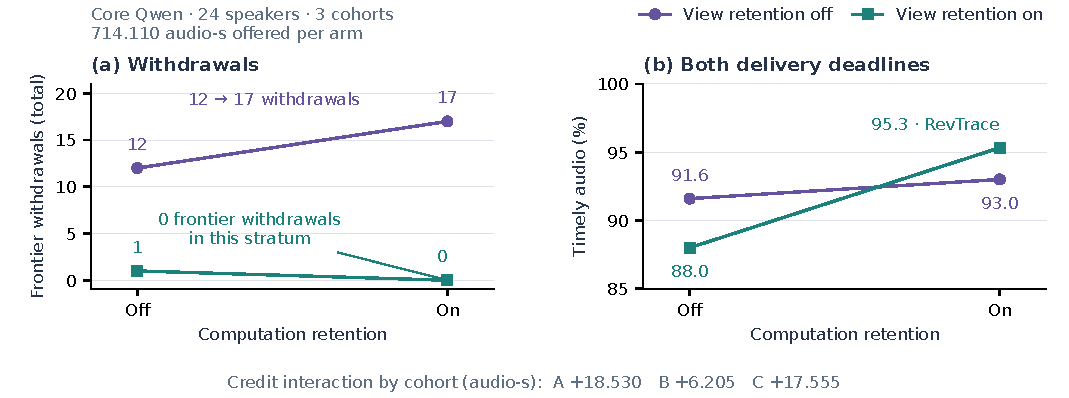
\includegraphics[width=\textwidth]{figures/core_interaction.pdf}
\caption{Factorial interactions in the predeclared Qwen, $\rho=1$,
staggered stratum. Points pool three eight-speaker cohorts;
each arm offers 714.110~s. (a) Total frontier withdrawals.
(b) Offered-audio fraction meeting display 2~s and certified 8~s deadlines.
Joint retention is RevTrace. All four arms and the Alternative joint
positive control fail whole-run D2 (15 runs).}
\label{fig:main_evidence}
\end{figure*}

Cohort-wise credit interaction,
$I=Y_{11}-Y_{10}-Y_{01}+Y_{00}$, is $+18.530$, $+6.205$, and $+17.555$~s.
These are three queue-coupled cohort contrasts, not independent deadline
windows. RevTrace's text remains revisable: 569 characters are erased
despite zero frontier withdrawal. Median per-run display P99 is 2.329~s,
above D2, so the benefit is retained progress under overload rather than
a whole-run service pass.

The Alternative joint implementation also yields zero withdrawals and 569
erased characters, with 667.530~s coverage and 2.534-s median P99. It
reproduces the supported-view behavior on the common substrate. Across
confirmation, 144 matched history groups and 22 positive-control pairs
agree on complete selected histories. Thus the comparison holds the
feedback task fixed while changing how valid work becomes service.
\par\noindent\textbf{Finding 1: retained computation does not ensure retained service.}
[EL] can retain work whose presentation a snapshot Consumer still removes.
Joint [EL]/[SUP] coordination preserves the supported ahead view.
